
\begin{frame}{Visión por Computadora}
%\begin{block}{Fundamentación} 
\begin{columns}
\begin{column}{0.60\textwidth}
    \begin{center}
\begin{itemize}
\item La visión por computadora imita la percepción humana y las capacidades de razonamiento.
\item Se intenta inferir conocimiento a partir de imágenes o videos.
\item Procesamiento de imágenes es una fase temprana de la VC. La entrada es una imagen y la salida es otra imagen.
\item En la visión por computadora, la entrada es una imagen pero la salida son datos. 
\end{itemize}
     \end{center}

\end{column}
\begin{column}{0.40\textwidth}  
    \begin{center}
     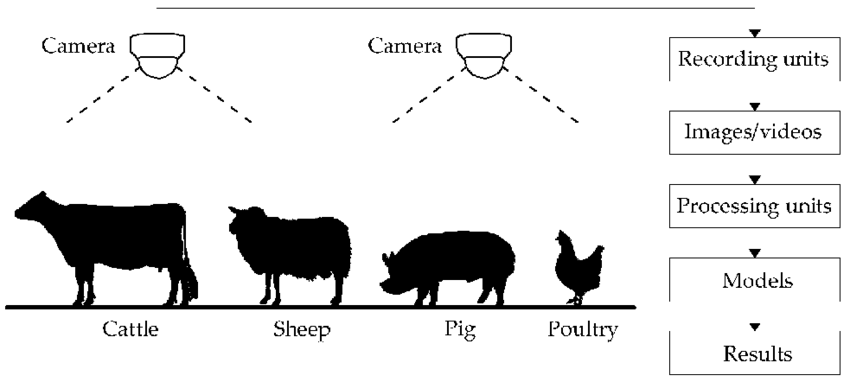
\includegraphics[width=0.9\textwidth]{Figs/VC}
     \end{center}
\end{column}
\end{columns}
%\end{block} 
\end{frame}

\begin{frame}{Visión por Computadora (Detección de Bordes) (II)}
  \begin{columns}
  \column {0.4\textwidth}
  \begin{itemize}
    \item La información acerca de bordes es útil para entender el ambiente.
    \item Las esquinas son primitivas que permiten identificar limites y puntos de interés dentro de la geometría de las imágenes.
  \end{itemize}  
      \column {0.3\textwidth}  
        \begin{center}
            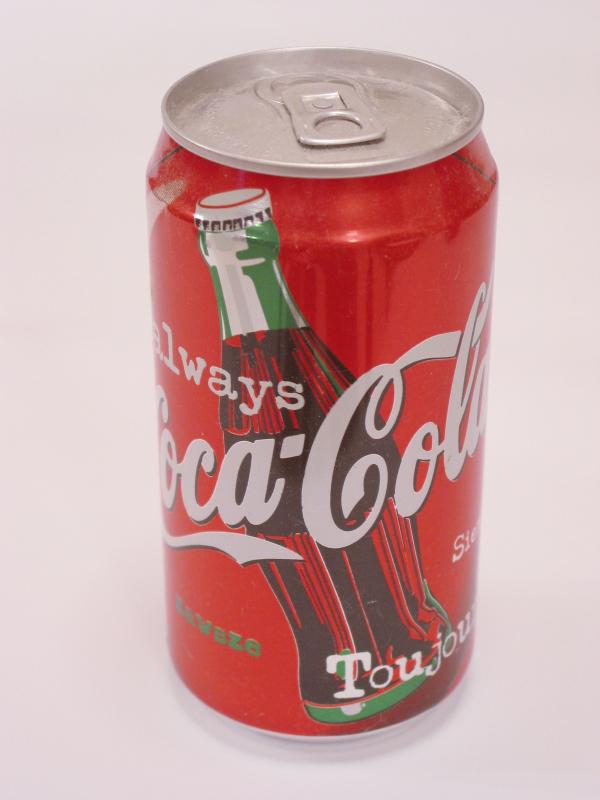
\includegraphics[width=\textwidth]{Figs/VC_CocaOrig}\\
     \end{center}
      
    \column {0.3\textwidth}  
        \begin{center}
            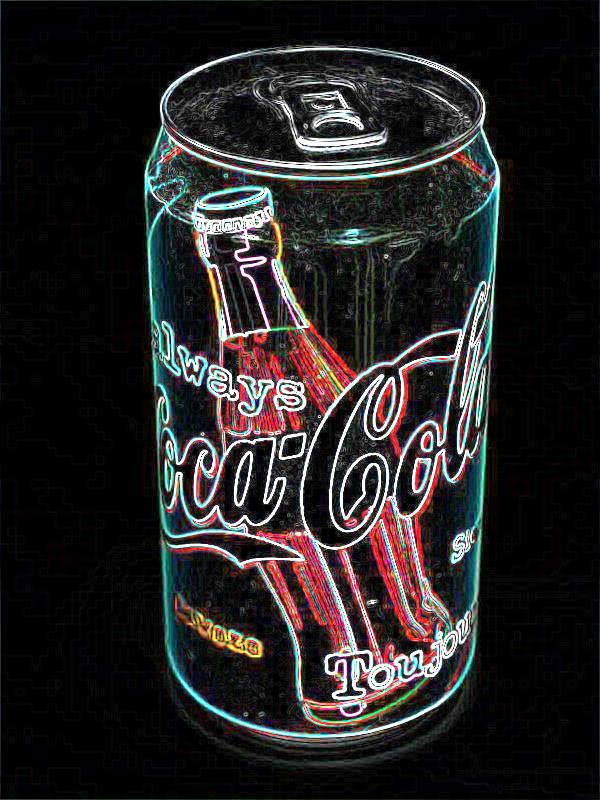
\includegraphics[width=\textwidth]{Figs/VC_CocaBordes}
     \end{center}

    \end{columns}

\end{frame}

\begin{frame}{Visión por Computadora (Segmentación) (II)}
\begin{columns}
  \column {0.8\textwidth}
  \begin{itemize}
    \item Localizar y aislar objetos de interés en la imagen.
    \item Localización de Objetivos, navegación, conteo de objetos
    \item Algoritmos de segmentación en escala de grises. Segmentación global (un umbral común para toda la imagen y segmentación local (umbrales múltiples en regiones de la imágen).
    \item Algoritmos de segmentación por color: muy utilizados para detectar la piel y encontrar partes del cuerpo.
  \end{itemize}
  
    \column {0.2\textwidth}  
        \begin{center}
            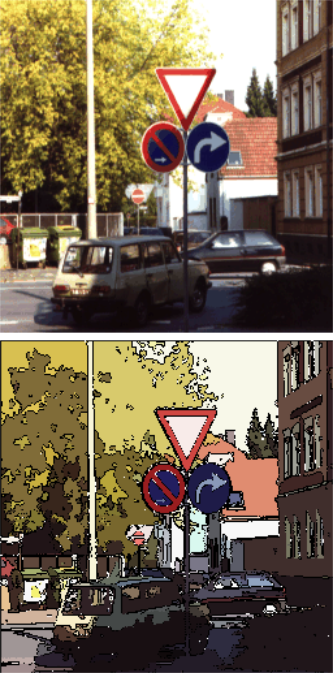
\includegraphics[width=\textwidth]{Figs/VC_Segmentacion}\\
     \end{center}

    \end{columns}
\end{frame}

\begin{frame}{Visión por Computadora (Template Matching) (II)}

Permite comparar imágenes aplicando operaciones de comparación entre regiones.
\begin{columns}
  \column {0.5\textwidth}
  \begin{itemize}
    \item Algoritmos clásicos basados en correlación: SAD, SSD, Rank.
	  \begin{itemize}
		    \item Ventajas: Facil de entender, rápidos
		    \item Desventajas: Sensibles a la escala, a rotaciones y a cambios en la iluminación. 
	  \end{itemize}
    \item Algoritmos modernos basados Aprendizaje Profundo
		\begin{itemize}
		    \item Ventajas: Buen desempeño 
		    \item Desventajas: Requieren de entrenamiento con muchas imágenes
	  \end{itemize}

  \end{itemize}
    \column {0.5\textwidth}  
        \begin{center}
            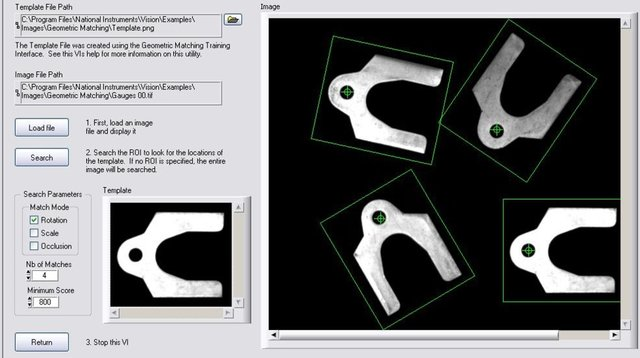
\includegraphics[width=\textwidth]{00_IntroComputerVision/figs/Industrial-software-example-for-Template-Matching_W640}\\
     \end{center}

    \end{columns}
\end{frame}


